\section{Participation notes 3}
Participant: Student

\begin{itemize}
    \item \textbf{Have them read the code-example} - Participant did not have any problem reading the code.
    \item \textbf{Have them draw the structure} - Initially the participant seemed confused by the question, but started drawing to explain the code structure. User represented the code as a conveyor belt with packages on top. the packages were the two functions being called by main. 
    \item \textbf{Have them submit the git URL} - User wrote in the URL and submitted. Participant then used the mouse for navigation and note that lines represent function calls and that the representation makes somewhat sense. 
    \item \textbf{Have them get the main() implementation} - Participant mentions that the participant does not know at all if task is possible, but continues for a while before clicking the function. Despite the implementation being shows, the participant is unaware and answers that participant does not know.
    \item \textbf{Participant visualization} \includepdf[pages={6}]{inc/generalAppendix/userStudies/participantsVisualization.pdf}
\end{itemize}